\section{Verification of Linear Models}
Since the system model consists of two models, \autoref{eq:model2S} and \ref{eq:firstModelLin}, the verification of the system model will be done in two steps. First, the individual models will be verified followed by a verification of the system model, where the two models are combined.
\subsection{Verification of Motors and Wheels Model}
First, \autoref{eq:model2S} is Laplace transformed to obtain a transfer function for the motors and wheel as follows: 
\begin{equation}
\frac{\Theta_w(s)}{V_a(s)} = \frac{2 \cdot k_t\cdot N_{ms}\cdot N_{sw}}{R_a(s^2(m_c \cdot r_w^2\cdot (N_{ms}\cdot N_{sw})^2 + 2 \cdot J_T) + s(2 \cdot\frac{k_t \cdot k_e}{R_a}+ 2\cdot B_T))}\label{eq:motorWheelTF}
\end{equation}

To be able to verify this linear model, parameter estimation is performed. It's purpose is to obtain a more precise model, as there may be deviations in the parameters, since there can uncertainties within the measurements. By using MATLAB it is possible to estimate parameters based on an initial guess. From this initial guess, MATLAB tunes the parameters to get a closer fit for the data. This fit is achieved by an optimization algorithm. By inserting the values found in \appref{motorMeasReport} and \appref{app:segwayParameters} into \autoref{eq:motorWheelTF} yields:

%To obtain the best result a system identification tool in MATLAB is used to estimated the model parameters, for the motors and wheels model. This tool require an initial guess, for which MATLAB tune the coefficients to get a better fit for the data. This fit is achieved by an optimization algorithm. By inserting the values found in \autoref{motorMeasReport} and \autoref{app:segwayParameters} into \autoref{eq:motorWheelTF} yields

\begin{align}
\frac{\Theta_w(s)}{V_a(s)}&=\frac{27.98}{s\cdot(s+20.29)}\\
\frac{\Omega_w(s)}{V_a(s)}&=\frac{27.98}{s+20.29}\label{eq:thomasA1}
\end{align}

Note that the second equation is obtained by simply multiplying the equation with an s, which corresponds to a differentiation. This is done since it is preferable to have the output of the transfer function as angular velocity instead of the angle, as the encoders measure the angular velocity.
\autoref{eq:thomasA1} is used as the initial guess for parameter estimation in MATLAB. To do parameter estimation, MATLAB needs pairs of a given input to the system and a measured output. The input should be chosen so that the dynamics of the system are seen. Here, the PWM input signal for the motors is chosen as the input signal, and is set to switch between the voltages 8.8 V and -8.8 V. The output is the angular velocity of the wheels. For MATLAB to perform parameter estimation, the model type is also needed. As previously mentioned, the motor is assumed to be a first order system, which is therefore used as the model type.

%This model is used as the initial guess for parameter estimation in Matlab. The data set that MATLAB is estimating based on, is where the motor voltage is changed from 8.8 V to -8.8 V, and the angular velocity of the wheel is measured, this can be seen in \autoref{fig:paramEst1}. 

\begin{figure}[H]
    \centering
    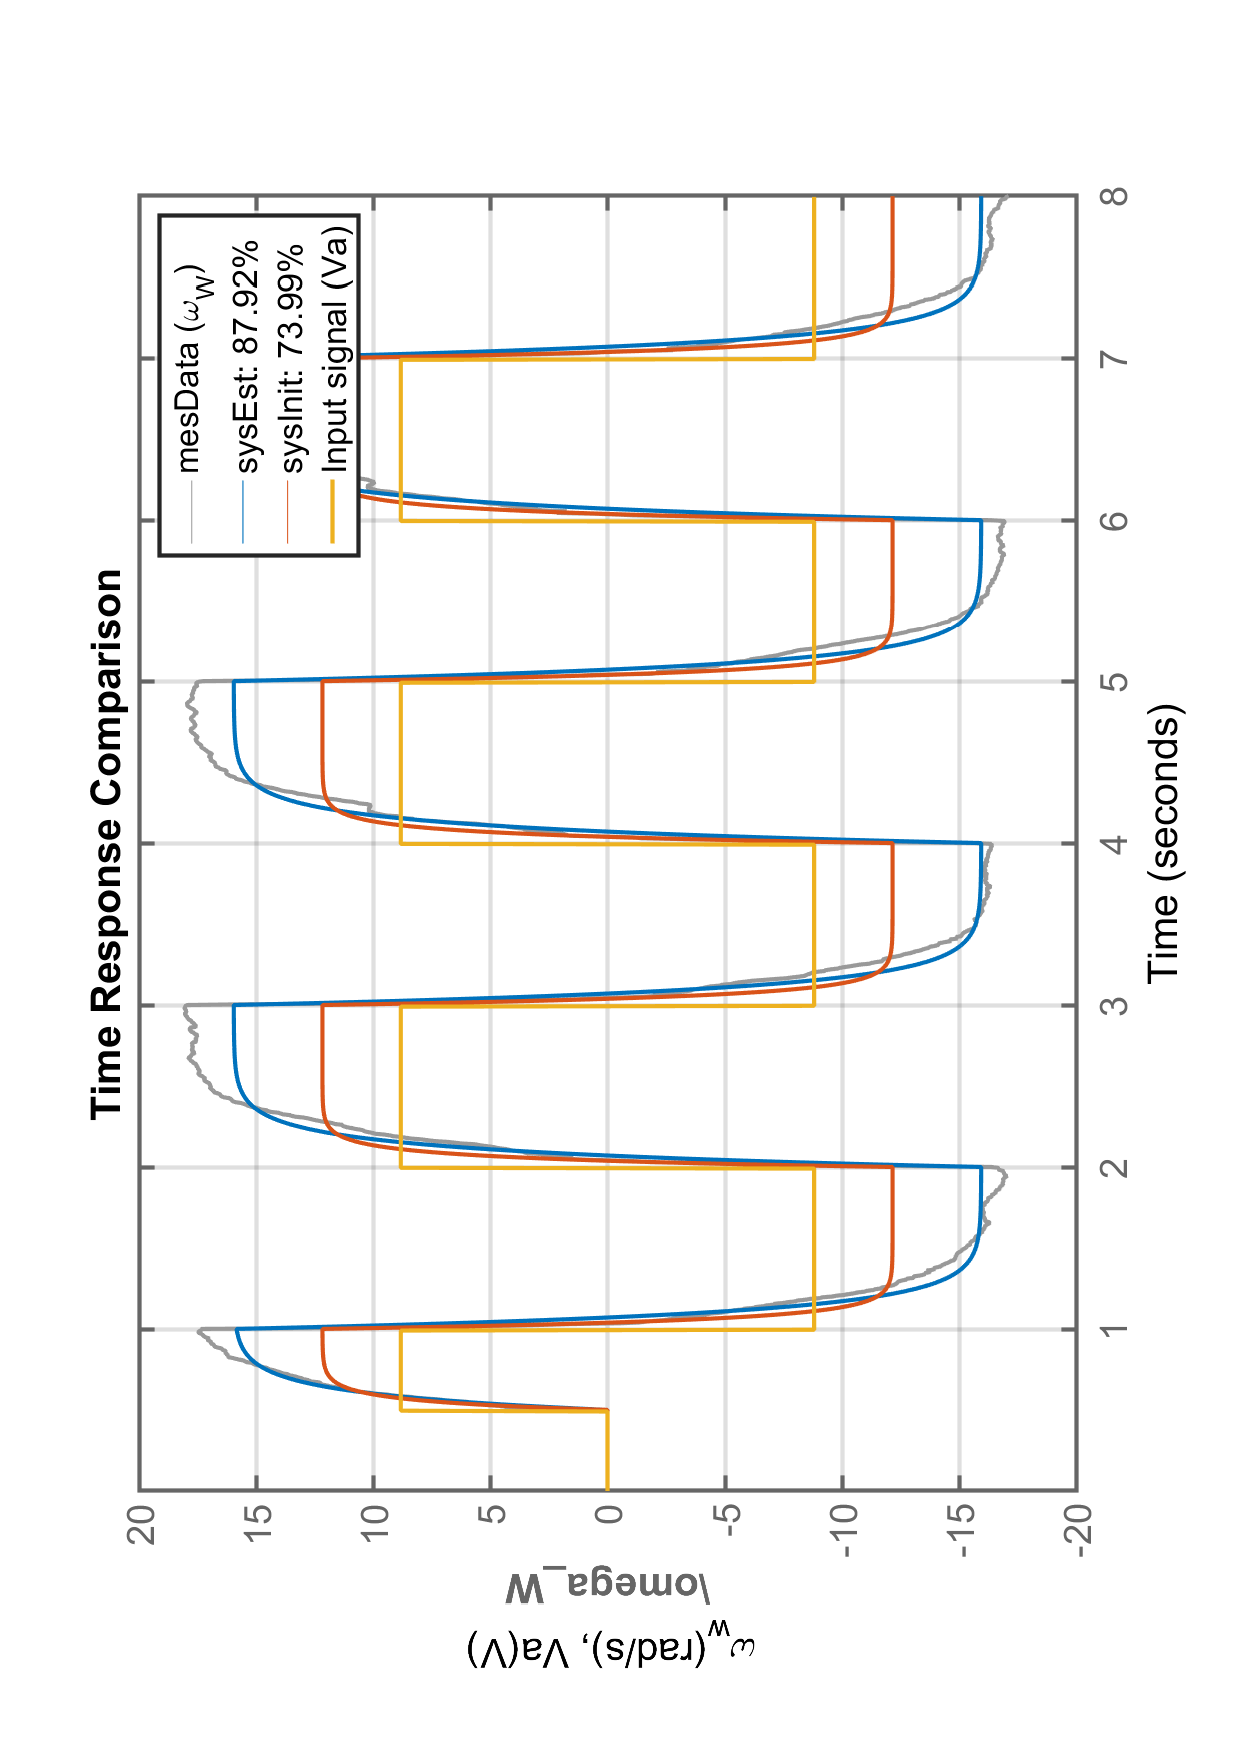
\includegraphics[height = 1\textwidth, angle = -90]{motorModelEst.pdf}
    \caption{Time response of both initial guess and optimized model based on given input and measured output.}
    \label{fig:paramEst1}
\end{figure} 

The response of the system over time can be seen in \autoref{fig:paramEst1}. The input signal is shown in yellow, and the output of the initial guess model is shown in orange, together with the measured data, which is shown in grey. The blue axis is MATLAB's estimate, based on the model type and measured data. The fit of 87.92 \% for the parameter estimation is considered acceptable, making the final model of the motors and wheels the following expression.
%The response can be seen in \autoref{fig:paramEst1}, where the initial guess' prediction, shown in orange, is shown together with the measured data in grey. The blue axis is MATLABs estimate, based on the model type and measured data, the input signal can be seen in a dark grey.
%The fit of 87.92\% is seen as very good and the final look on of the model is thereby determined as:
\begin{equation}
\frac{\Omega_w(s)}{V_a(s)}=\frac{17.72}{s+9.799}
\end{equation}

\subsection{Verification of Inverted Pendulum Model \label{sec:varificationpen}}
To verify the inverted pendulum model, a transfer function where $\Theta_w(s)$ is input and $\Theta_p(s)$ is output, needs to be derived. Thus \autoref{eq:firstModelLin} has to be Laplace transformed as well as rearranged to obtain the desired transfer function:
\begin{equation}
\frac{\Theta_p(s)}{\Theta_w(s)} = \frac{m_p \cdot l \cdot r_w \cdot s^2}{s^2 (J_p + m_p \cdot l^2) - m_p \cdot l \cdot g}\label{eq:penLinTF}
\end{equation}

The model for the inverted pendulum, \autoref{eq:penLinTF}, is to be verified by turning the segway upside down and reversing the gravity in the model expression. This has the implications of the system becomes stable, which is necessary for parameter estimation to work. The segway is then moved on rails and the pendulum angle is measured with $\theta_p(t) = 0$ being downwards instead of upwards. This means that from a modelling perspective, the only thing changed is the direction of gravity. By inserting the values found in \autoref{motorMeasReport} and \autoref{app:segwayParameters} into \autoref{eq:penLinTF} yields:

%The model for the inverted pendulum, \autoref{eq:penLinTF}, is verified by turning the segway around and reversing the gravity in the model. This have the implications of the system becoming stable. The segway is then moved on rails and the angle is measured with zero being downwards instead of up so model wise the only thing changed is gravity. By inserting the values found in \autoref{motorMeasReport} and \autoref{app:segwayParameters} into \autoref{eq:penLinTF} yields:
\begin{align}
\frac{\Theta_p(s)}{\Theta_w(s)}&=\frac{0.09217\cdot s^2}{s^2 + 15.47}\\
\frac{\Theta_p(s)}{\Omega_w(s)}&=\frac{0.09217\cdot s}{s^2 + 15.47}
\end{align}
Note that as for the motors and wheels model's output, the input of this transfer function is the angular velocity of the wheel instead of the the angular position of the wheel.
This is put through MATLAB's system identification tool as explained previously, from which the results can be seen in \autoref{fig:paramEst2}. An input delay is used even though no delay is seen in the model, which is done to get a better fit. 

%\begin{equation}
%\frac{\theta_p(s)}{\omega_w(s)}=\frac{0.04609\cdot s}{s^2 + 15.47}
%\end{equation}

%The verification of this model was first done on a wrong foundation, due to a implementation error in Simulink, because of this the fit that the control chapter is using is not optimal. 

\begin{figure}[H]
    \centering
    %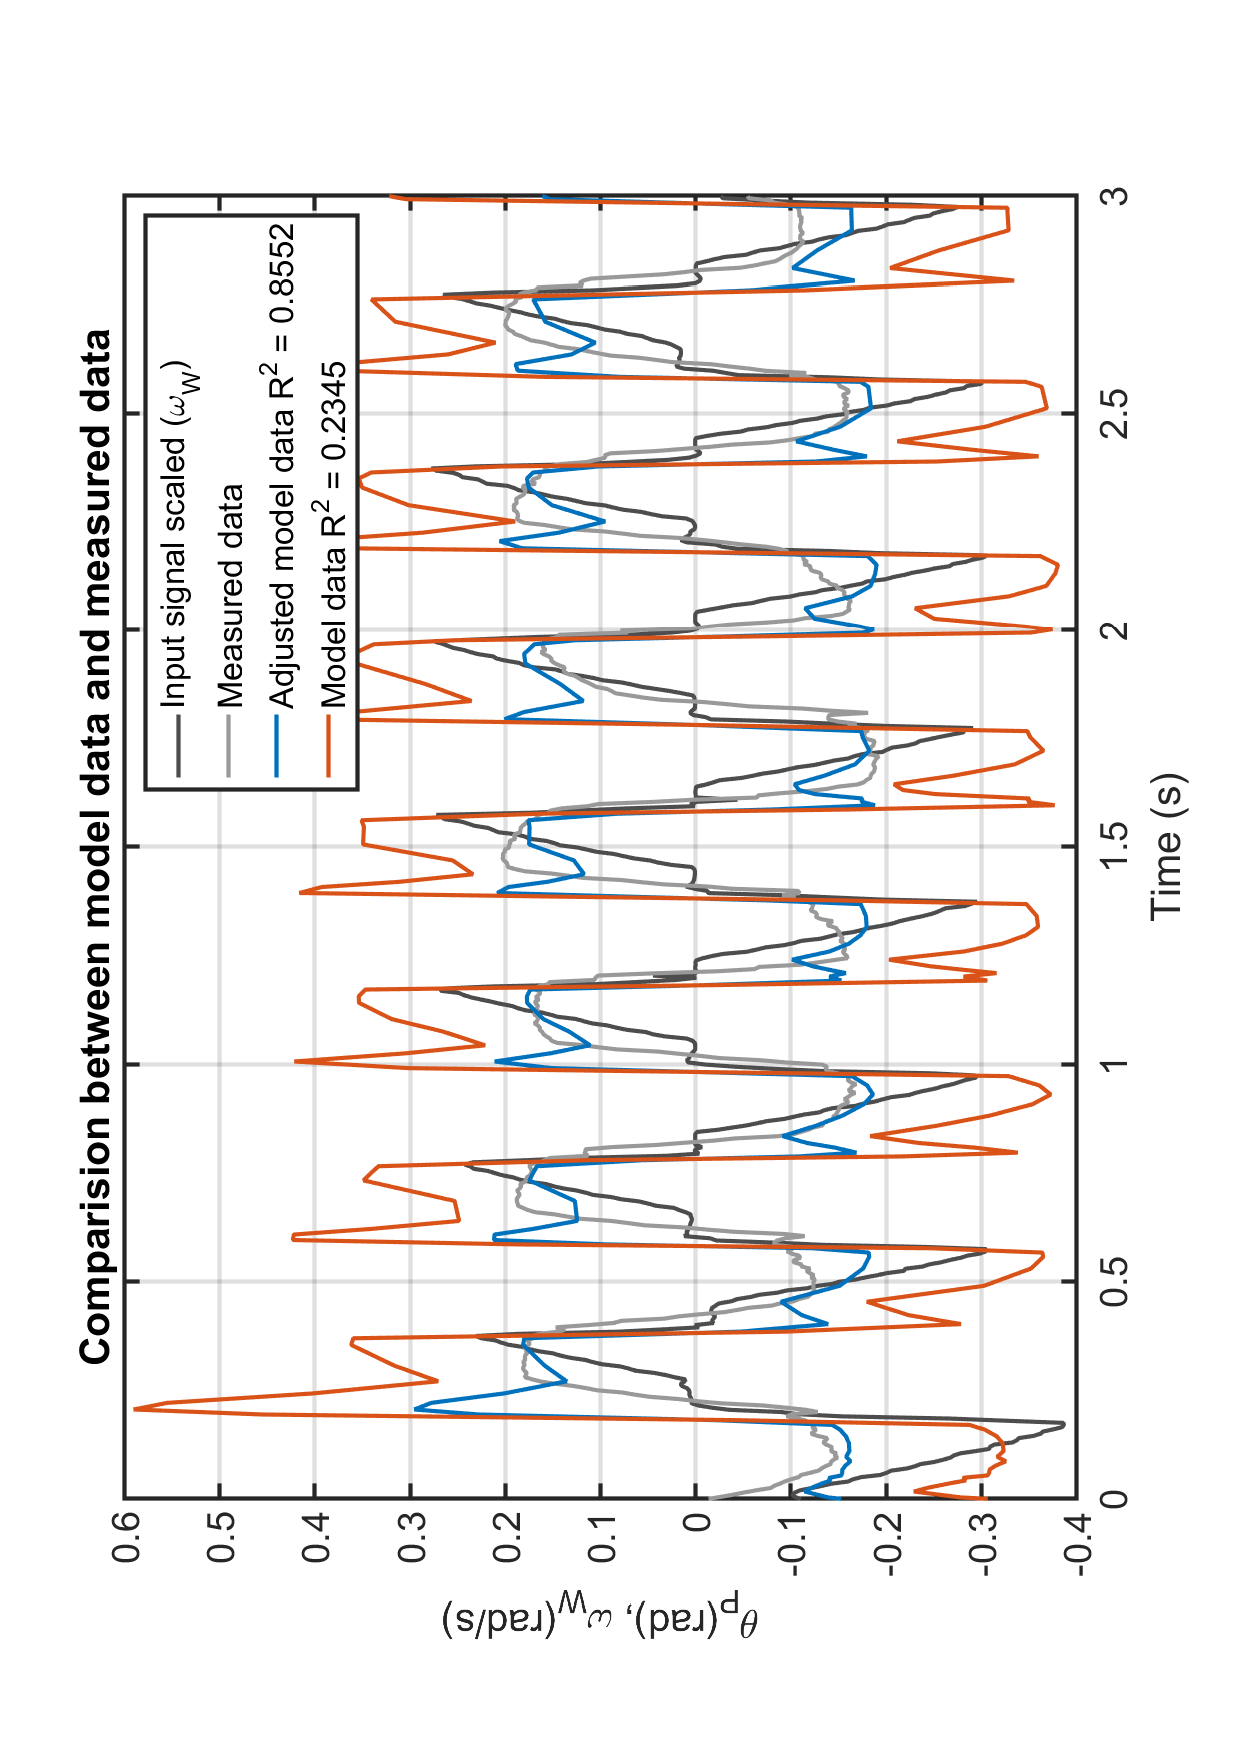
\includegraphics[height = 0.9\textwidth, angle = -90]{modelComparison.pdf}
    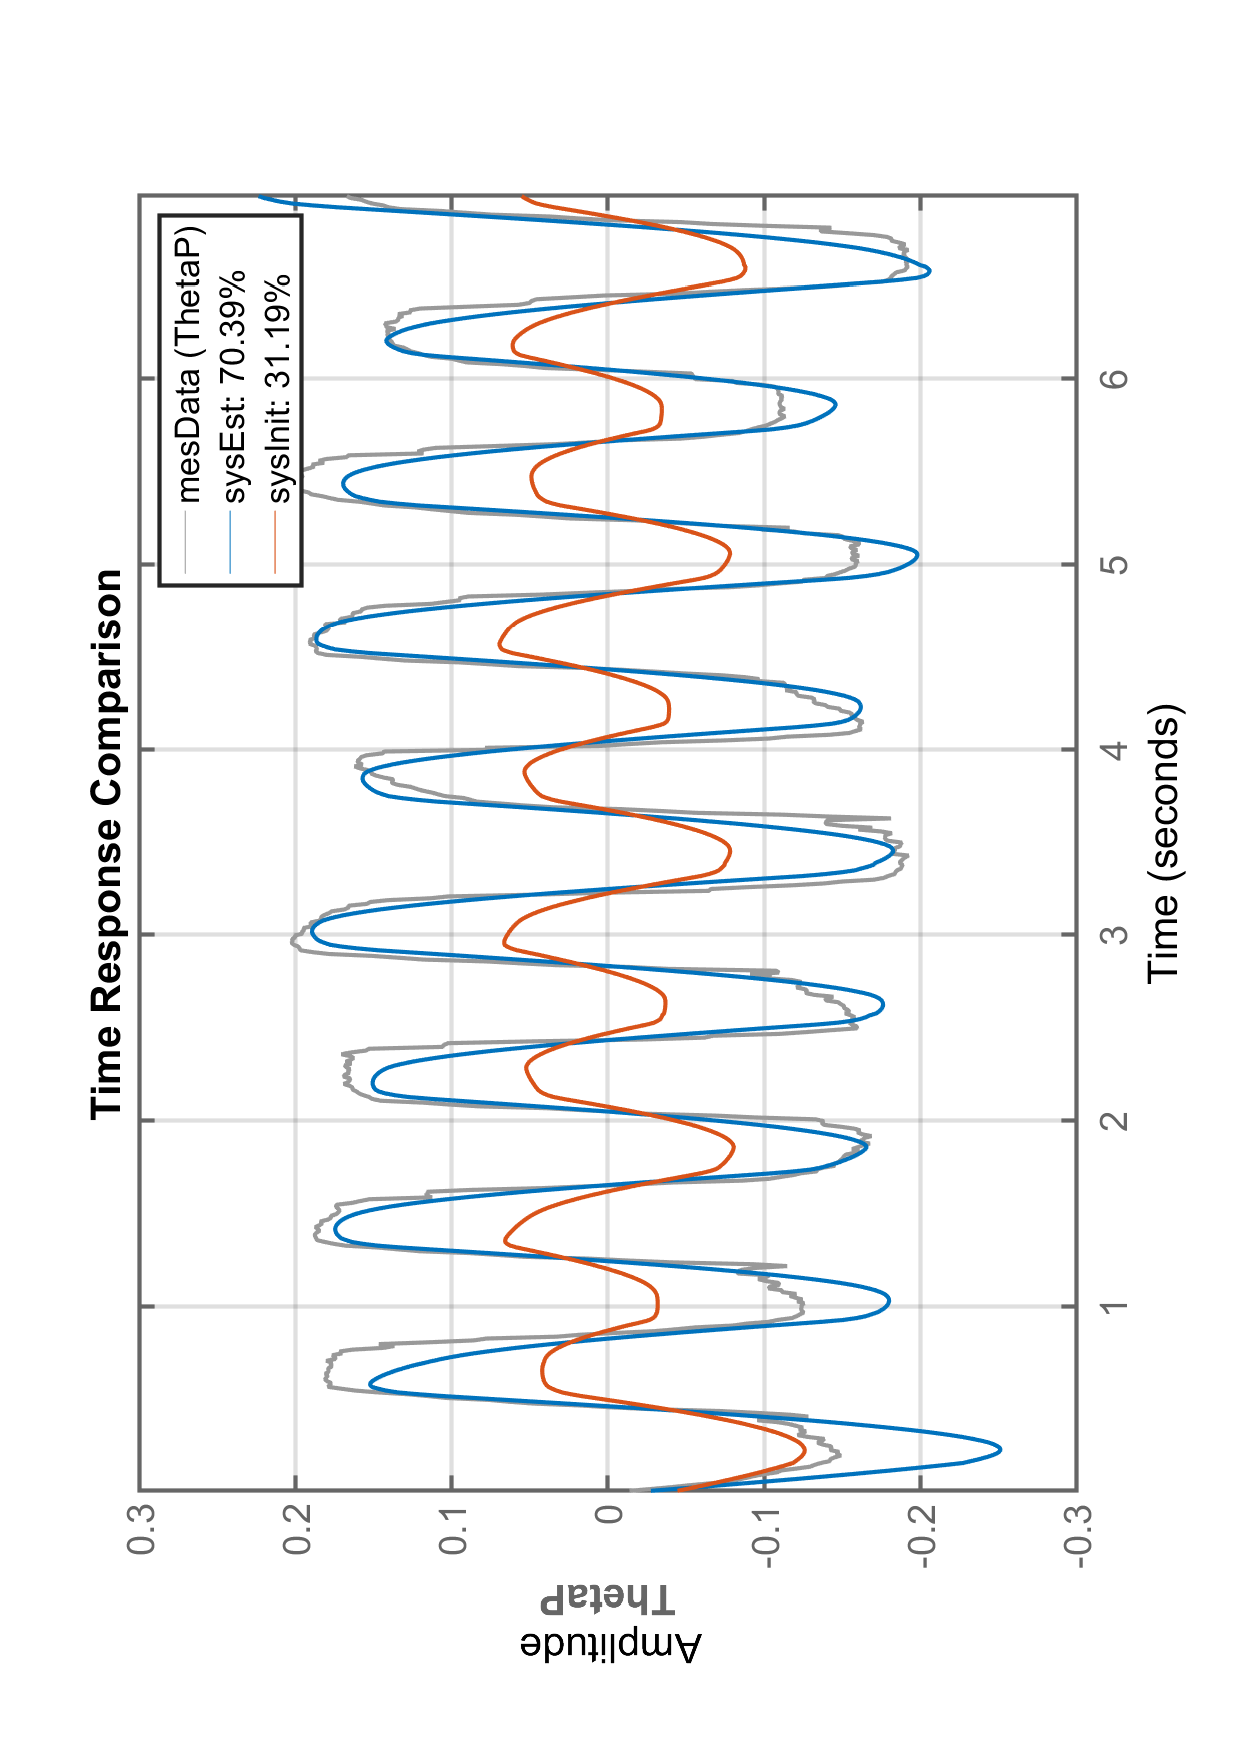
\includegraphics[height = 1\textwidth, angle = -90]{pend2.pdf}
\vspace{-0.3 cm}    
    \caption{Time response of inverted pendulum model.}
    \label{fig:paramEst2}
\end{figure} 
\vspace{-1 cm}
From \autoref{fig:paramEst2} it can be seen that a fairly big change happens to the output and fit of the system. This is seen as a problem, due to the fact that most of the parameters in the transfer function are lengths and masses, which are quite simple to measure without a lot of uncertainties. A possible cause for this discrepancy is that the model may not include enough factors to represent reality adequately, but due to time constraints it is not possible to review the model further, and therefore the sysEst provided by MATLAB will be used for controller design. A concern is also that this sysEst fits this exact set of data, which only represent one type of input. After reversing gravity again, to describe the unstable system, the transfer function for the inverted pendulum model becomes:
\begin{equation}
	\frac{\theta_p(s)}{\omega_w(s)}=\frac{0.2367\cdot s}{s^2 - 21.92}
\end{equation}
\subsection{Verification of Segway Model}
To verify the linear system model, the two newly derived models from the two previous sections are multiplied and compared to both the system model and the measured data. The data is measured in the same way as the inverted pendulum model verification. The comparison is done in Simulink where the system is simulated, and the results can be seen in \autoref{fig:paramEst3}.

\begin{figure}[H]
    \centering
    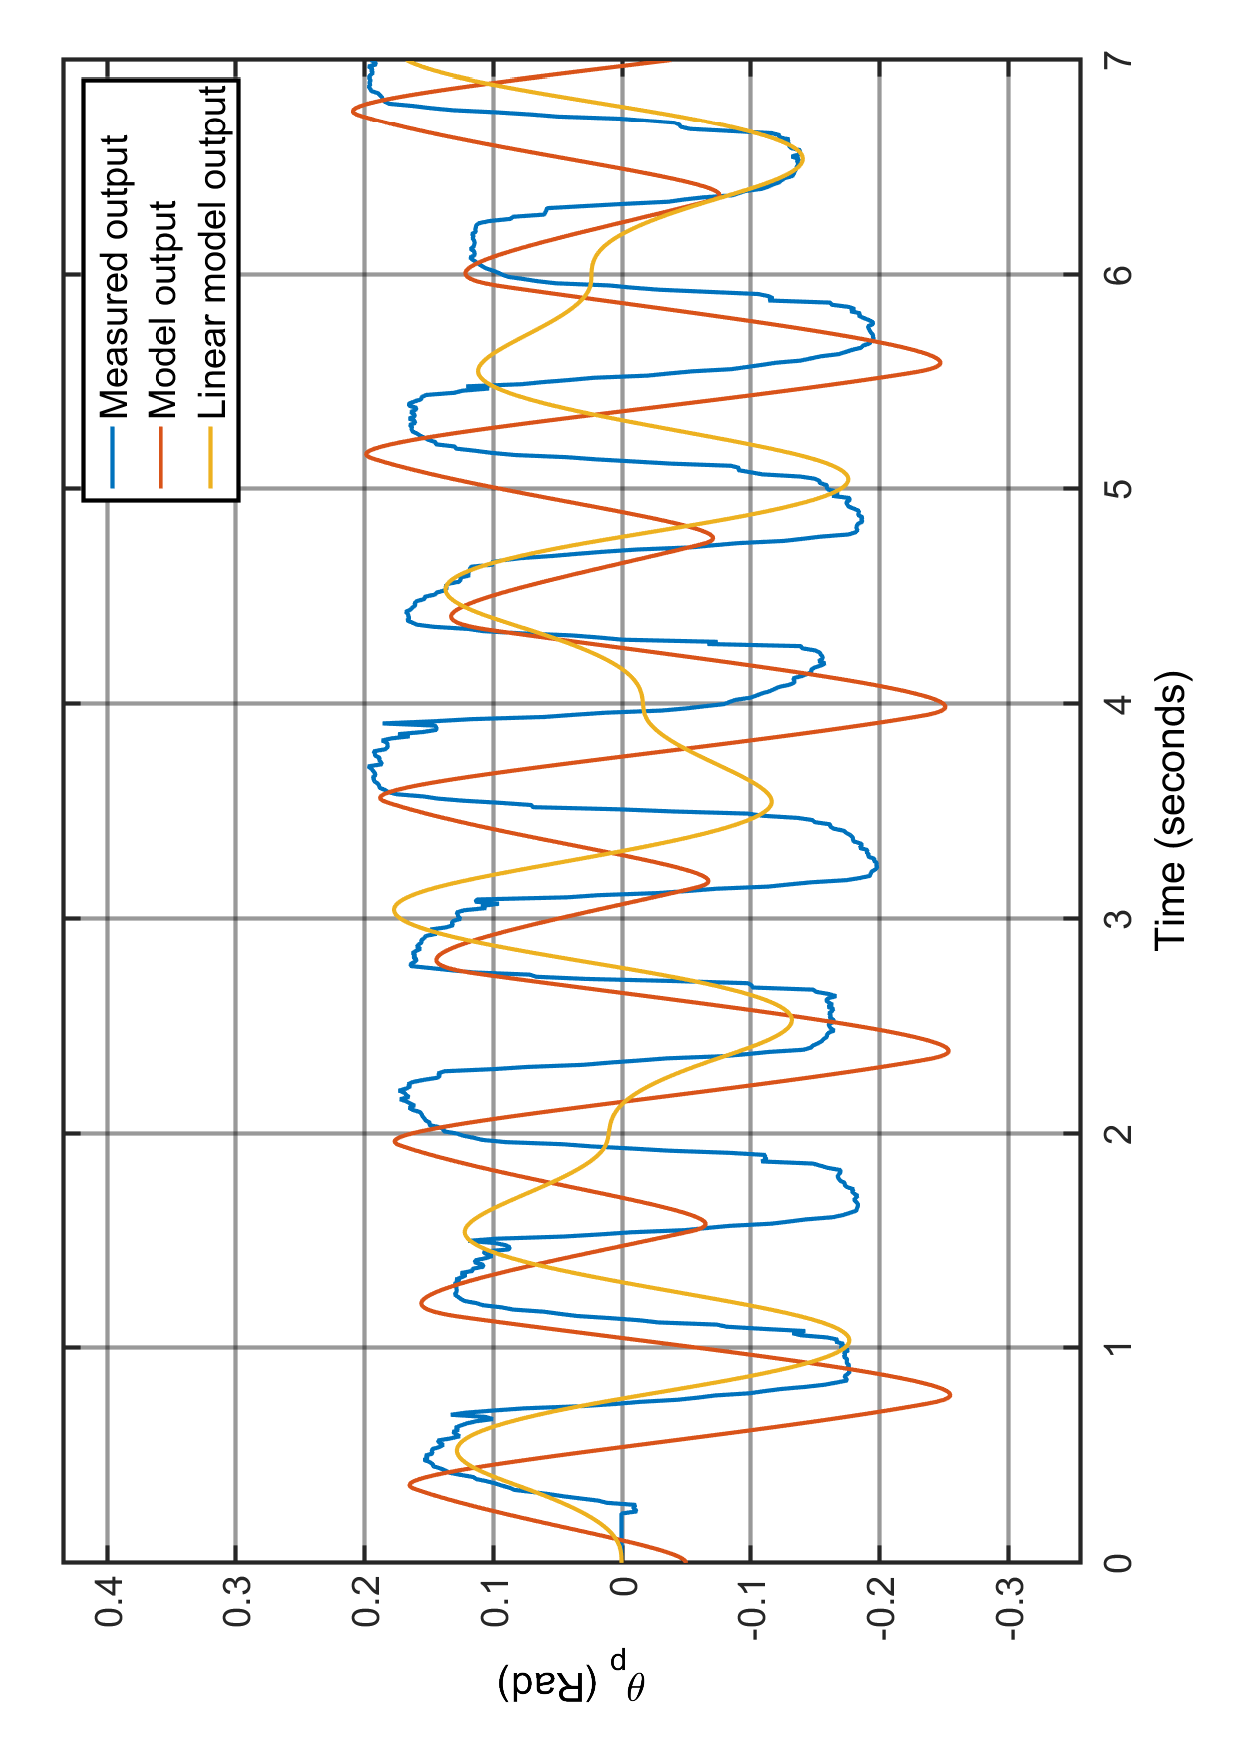
\includegraphics[height = 0.88\textwidth, angle = -90]{sys2.pdf}
    \caption{Time response of system model and linear model compared to measured data.}
    \label{fig:paramEst3}
\end{figure} 
%From \autoref{fig:paramEst3} it can be seen that the fit between the models and reality is poor. It is believed to be for the same reasons as mentioned in \autoref{sec:varificationpen}, but due to time constraints, a controller design will be based upon these models, despite the poor fit.
\vspace{-0.7 cm}
From \autoref{fig:paramEst3} it can be seen that the fit between the models and reality is poor. It is believed to be for the same reasons as mentioned in \autoref{sec:varificationpen}, but could also be due to implementation errors in Simulink, which due to time constraints are not further investigated. A controller design will be based upon these models, despite this poor fit.

Now that the transfer function for the segway is found, it can be used for the controller design, which is done in the following chapter. 
%A transfer function describing the entire system of the segway is now formed as shown in \autoref{fig:modelOverallLin}. This is done by combining \autoref{eq:motorWheelTF} with \autoref{eq:penLinTF}.
%\begin{equation}
%\frac{\Theta_p(s)}{V_a(s)} = \frac{\Theta_w(s)}{V_a(s)} \cdot \frac{\Theta_p(s)}{\Theta_w(s)} = \frac{K_1 \cdot s}{s^3 \cdot K_2 + s^2 \cdot K_3 - s \cdot K_4 - K_5}\label{eq:segwayTF}
%\end{equation}
%%Where the K constants are representing the following term:\\
%\begin{where}
%\begin{tabular}{p{40pt} l}
%& $K_1=k_t \cdot m_p \cdot l \cdot r_w \cdot N_{ms}\cdot N_{sw}$\\
%& $K_2=R_a\cdot (\frac{1}{2}\cdot m_c \cdot r_w^2\cdot (N_{ms}\cdot N_{sw})^2 +  J_T)(J_p + m_p \cdot l^2)$\\
%& $K_3=(k_t \cdot k_e + R_a \cdot B_T)(J_p + m_p \cdot l^2)$\\
%& $K_4=R_a\cdot m_p\cdot l \cdot g\cdot (\frac{1}{2}\cdot m_c \cdot r_w^2\cdot (N_{ms}\cdot N_{sw})^2 +  J_T)$\\
%& $K_5=(k_t \cdot k_e + R_a \cdot B_T)\cdot m_p\cdot l \cdot g$\\
%\end{tabular}
%\end{where}